% mnnit.cls (2005) replaces LaTeX's float macro with an old version that
% breaks every figure/table on current LaTeX. Keep the kernel version and
% only add the single spacing inside floats that the class intended.
\makeatletter\let\kernel@xfloat\@xfloat\makeatother
\documentclass{mnnit}
\makeatletter
\let\@xfloat\kernel@xfloat
\g@addto@macro\@floatboxreset{\def\baselinestretch{1}\normalsize}
\makeatother
\setcitestyle{numbers,square}

% Standard packages only (available on Overleaf / TeX Live / MiKTeX).
\usepackage{amsmath}
\usepackage{amssymb}
\usepackage{graphicx}
\usepackage{booktabs}
\usepackage{array}
\usepackage{adjustbox}
\graphicspath{{figures/}}
% Let TeX stretch a line rather than push long code words into the margin.
\setlength{\emergencystretch}{3em}

% Notation used throughout the report.
\providecommand{\ket}[1]{\left|#1\right\rangle}
\providecommand{\bra}[1]{\left\langle#1\right|}
\newcommand{\cq}{C$\rightarrow$Q}
\newcommand{\qc}{Q$\rightarrow$C}
\newcommand{\expval}[1]{\left\langle #1\right\rangle}

% ---------------------------------------------------------------------------
% Undertaking and Certificate pages.
% The class versions use fixed 3 cm / 5 cm gaps sized for a single author;
% with four authors the heading ends up alone on one page and the text on the
% next. These versions keep the class wording (in plural, for a team), use the
% same chapter-style heading as the other front-matter pages, and fit on one
% page each.
% ---------------------------------------------------------------------------
\newcommand{\teamnames}{Saksham Tiwari (20233243), Prajjwal Singh (20233213),
Madipelli Rithvik (20233176) and Sanchari Ray (20233250)}
\newcommand{\signline}[1]{%
  \parbox[t]{0.42\linewidth}{\centering
    \rule{0.85\linewidth}{0.4pt}\\[2pt] #1}}
\makeatletter
\renewcommand{\undertakingpage}{%
  \chapter*{Undertaking}
  We declare that the work presented in this report titled
  ``{\sl\@title}'', submitted to the \mbox{\@dept} Department, \@college,
  for the award of the \textbf{\emph{\@degree}} degree in
  \textbf{\emph{\@specialization}}, is our original work. We have not
  plagiarized or submitted the same work for the award of any other degree.
  In case this undertaking is found incorrect, we accept that our degree may
  be unconditionally withdrawn.

  \vspace{1.5cm}
  \noindent\@submitdate\\
  Allahabad

  \vspace{2cm}
  \noindent
  \signline{Saksham Tiwari\\(20233243)}\hfill
  \signline{Prajjwal Singh\\(20233213)}\\[2cm]
  \signline{Madipelli Rithvik\\(20233176)}\hfill
  \signline{Sanchari Ray\\(20233250)}
}
\renewcommand{\signaturepage}{%
  \chapter*{Certificate}
  Certified that the work contained in the report titled ``{\sl\@title}'',
  by \teamnames, has been carried out under my supervision and that this
  work has not been submitted elsewhere for a degree.

  \vspace{3cm}
  \noindent\@submitdate\hfill
  \parbox[t]{0.55\linewidth}{\centering
    \rule{0.65\linewidth}{0.4pt}\\[2pt]
    (\@supervisor)\\
    \@dept\ Department\\
    M.N.N.I.T. Allahabad}
}
\makeatother

\begin{document}
\title{Hybrid Quantum--Classical Neural Networks for Tuberculosis Detection from Chest X-ray Images}
\author{Saksham Tiwari (20233243)\\
Prajjwal Singh (20233213)\\
Madipelli Rithvik (20233176)\\
Sanchari Ray (20233250)}
\supervisor{Dr. Rajitha B.}

\specialization{Computer Science \& Engineering}
\figurespagetrue
\tablespagetrue
\beforepreface

\prefacesection{Preface}
This report describes a B.Tech.\ project that asks a narrow, testable
question: when a small quantum circuit is inserted into an image classifier,
does the classifier get better, and does it matter where the circuit is
placed? We study the question on a real medical task, the detection of
tuberculosis from chest radiographs, using circuits of four to ten qubits
that are simulated on a laptop CPU.

The project combines the two halves of the subject in equal measure. On the
quantum side it implements a variational quantum classifier, a quantum
convolution (``quanvolution'') layer, two data-encoding schemes and three
entanglement patterns, and it measures the circuits themselves:
expressibility, entangling capability, gradient scaling with qubit count and
robustness to hardware noise. On the machine-learning side it builds a
reproducible pipeline with fixed data splits, repeated seeds, matched
classical controls, low-data experiments and paired statistical tests, so
that every claim about the quantum components can be checked against a fair
classical alternative.

The code, the configuration of every experiment and all raw results are
included with this report so that each number in it can be regenerated.

\prefacesection{Acknowledgements}
We express our sincere gratitude to our project supervisor,
Dr. Rajitha B., for the guidance, encouragement and critical feedback
given throughout this project. The supervisor's insistence on fair
comparisons and honest reporting shaped the way every experiment in this
report was designed.

We thank the Department of Computer Science and Engineering, Motilal Nehru
National Institute of Technology Allahabad, Prayagraj, for providing the
academic environment and resources that made this work possible, and the
faculty members whose courses in machine learning and quantum computing
laid its foundation.

We are grateful to the authors of the TB Chest X-ray Database for making
their data publicly available, and to the developers of PyTorch and
PennyLane, whose open-source software was used for every experiment.

Finally, we thank our families and friends for their constant support.

\vspace{1cm}
\begin{flushright}
Saksham Tiwari (20233243)\\
Prajjwal Singh (20233213)\\
Madipelli Rithvik (20233176)\\
Sanchari Ray (20233250)
\end{flushright}

\prefacesection{Abstract}
Tuberculosis (TB) remains one of the leading infectious causes of death
worldwide, and chest radiography is a standard first-line screening tool.
This project investigates whether hybrid quantum--classical neural networks
can improve automated TB detection, and compares two ways of combining the
paradigms: a classical$\rightarrow$quantum (\cq) model, in which a
convolutional neural network (CNN) feeds a four-qubit variational quantum
classifier, and a quantum$\rightarrow$classical (\qc) model, in which a
quantum convolution filter processes $2\times2$ pixel patches before a CNN.
Both are evaluated on the TB Chest X-ray Database (3,500 normal and 700 TB
images at $64\times64$) against a CNN baseline and four classical controls
matched in structure and size, with circuits simulated in PennyLane.

On the full training set the \cq{} hybrid reached $98.41 \pm 0.32\%$
accuracy and an F1-score of $0.952 \pm 0.010$ over three seeds, compared with
$97.67 \pm 0.33\%$ and $0.930 \pm 0.009$ for the classical CNN and
$97.72 \pm 0.40\%$ and $0.930 \pm 0.012$ for a parameter-matched classical
head. With an ImageNet-pretrained ResNet18 backbone the quantum head reached
$99.47 \pm 0.18\%$ accuracy. The improvements are consistent across seeds
but not statistically significant in paired McNemar tests ($p \geq 0.09$).
The \qc{} hybrid matched the full CNN with about four times fewer
parameters, but so did plain classical downsampling. Circuit analysis
showed that the entangling layers approach Haar-random
expressibility at depth two to three, that gradient variance decays roughly
exponentially with qubit count, and that the trained hybrid keeps its
accuracy with only ten measurement shots and under depolarising noise up to
$p = 0.2$ per layer. At today's simulable scale, quantum layers are a
viable, noise-robust component of a medical image classifier, but not yet a
demonstrably superior one.

\prefacesection{List of Abbreviations}
\begin{tabular}{@{}ll@{}}
AUC & Area Under the (ROC) Curve \\
BCE & Binary Cross-Entropy \\
BP & Barren Plateau \\
\cq & Classical-to-Quantum hybrid (CNN features $\rightarrow$ quantum circuit) \\
CNN & Convolutional Neural Network \\
CNOT & Controlled-NOT gate \\
CXR & Chest X-ray (radiograph) \\
FN / FP & False Negative / False Positive \\
KL & Kullback--Leibler divergence \\
NISQ & Noisy Intermediate-Scale Quantum \\
PQC & Parameterised Quantum Circuit \\
\qc & Quantum-to-Classical hybrid (quantum convolution $\rightarrow$ CNN) \\
QML & Quantum Machine Learning \\
ROC & Receiver Operating Characteristic \\
SEL & StronglyEntanglingLayers (circuit template) \\
TB & Tuberculosis \\
VQC & Variational Quantum Circuit / Classifier \\
\end{tabular}

\afterpreface

\chapter{Introduction}
\label{ch:intro}

\section{Motivation}
Tuberculosis is caused by the bacterium \emph{Mycobacterium tuberculosis}
and most often affects the lungs. According to the World Health
Organization, it was again the world's leading cause of death from a single
infectious agent in 2023, with an estimated 10.8 million people falling ill
and about 1.25 million deaths~\cite{who2024}. India carries the largest
share of the global burden, which makes early and cheap detection a
public-health priority in our own context.

Chest radiography is one of the main tools for TB screening. It is fast and
inexpensive, but every image must be read by a trained radiologist, and in
high-burden regions radiologists are scarce. The WHO therefore recommends
computer-aided detection software as an option for screening
adults~\cite{who2021screening}, and an independent evaluation of five
commercial products in Bangladesh found that all of them outperformed
experienced radiologists at the operating points studied~\cite{qin2021}.

Such systems are built on convolutional neural networks
(CNNs)~\cite{lecun1998}. Since a deep CNN won the ImageNet
challenge~\cite{krizhevsky2012, deng2009}, deep learning has become the
standard approach in computer vision~\cite{lecun2015} and in medical image
analysis~\cite{litjens2017}; large public collections such as
ChestX-ray8~\cite{wang2017} made it possible to train radiograph classifiers
that approach radiologist-level performance~\cite{rajpurkar2017}. For TB,
ImageNet-pretrained CNNs reach accuracies in the high nineties on public
datasets~\cite{rahman2020}.

Quantum computing offers a different model of computation. Feynman observed
that quantum systems are exponentially expensive to simulate
classically~\cite{feynman1982}; Shor's factoring algorithm~\cite{shor1997}
and Grover's search algorithm~\cite{grover1996} showed provable speed-ups
for specific problems; and in 2019 a 53-qubit processor performed a sampling
task argued to be beyond classical supercomputers~\cite{arute2019}. Present
devices, however, belong to the \emph{noisy intermediate-scale quantum}
(NISQ) era~\cite{preskill2018}: they have few qubits and every gate adds
noise. The dominant NISQ approach to machine learning is the
\emph{variational quantum circuit}, a short circuit with trainable rotation
angles optimised by a classical computer like the weights of a neural
network~\cite{schuld2020circuit, mitarai2018, farhi2018, benedetti2019}. The
same principle underlies the variational quantum
eigensolver~\cite{peruzzo2014, kandala2017}; the family of methods is
reviewed in~\cite{cerezo2021vqa, schuld2018book}.

Because current devices are small, practical models are \emph{hybrid}: a
classical network handles the high-dimensional image and a small circuit is
inserted at one point. In \emph{classical-to-quantum} transfer learning a
CNN compresses the image into a few features that a circuit
classifies~\cite{mari2020}; in a \emph{quanvolutional} network a circuit is
slid over the image like a convolution filter~\cite{henderson2020}.
PennyLane~\cite{bergholm2018} makes both kinds of model ordinary
PyTorch~\cite{paszke2019} modules that can be trained by backpropagation
through a simulator.

\section{Problem Statement}
Published hybrid models are often compared only with a classical model of
a different size or structure, on a single run, so it is hard to tell
whether the quantum circuit is responsible for the result. This project
asks:

\begin{quote}
\emph{Does adding a small quantum circuit improve a CNN classifier for
tuberculosis detection from chest X-rays, and does the answer depend on
whether the circuit is placed after the classical feature extractor (\cq)
or before it (\qc), once each hybrid is compared with a classical model of
the same structure and size?}
\end{quote}

\section{Objectives and Contributions}
The objectives were to build a reproducible pipeline for the TB Chest X-ray
Database; to implement a classical CNN baseline, a \cq{} hybrid and a \qc{}
hybrid together with classical controls matched to each hybrid; to study
the effect of circuit design, backbone and training-set size with repeated
seeds and paired statistical tests; and to analyse the circuits themselves.
The main contributions are:
\begin{enumerate}
  \item A configurable PyTorch--PennyLane code base in which every
        experiment differs from its reference in exactly one setting.
  \item A comparison of both hybrid placements with a baseline and four
        matched controls on five training-set sizes and three seeds
        (105 training runs), a 12-configuration circuit ablation, and a
        backbone $\times$ head study including pretrained ResNet18.
  \item A quantitative analysis of the circuits: expressibility,
        entangling capability, barren-plateau scaling, and robustness to
        finite shots and depolarising noise.
  \item An honest assessment: the \cq{} hybrid is consistently but not
        significantly better than its controls, and the \qc{} hybrid's
        parameter efficiency is reproduced by classical downsampling.
\end{enumerate}

Chapter~\ref{ch:related} reviews the background and related work,
Chapter~\ref{ch:proposed} describes the data, models and protocol,
Chapter~\ref{ch:results} presents and analyses the results, and
Chapter~\ref{ch:conclusion} concludes.

\chapter{Related Work}
\label{ch:related}

\section{Convolutional Neural Networks}
\label{sec:rw_cnn}
A CNN applies small learned filters across the whole image~\cite{lecun1998}.
A convolutional layer with $C_{\mathrm{in}}$ input channels,
$C_{\mathrm{out}}$ output channels and a $k \times k$ kernel has
$C_{\mathrm{out}}(C_{\mathrm{in}}k^2 + 1)$ parameters, independently of the
image size, and recognises a feature wherever it appears. Each convolution
is followed by a non-linearity, usually $\mathrm{ReLU}(z) = \max(0,
z)$~\cite{nair2010}, and by pooling that reduces the resolution; fully
connected layers then map the features to class scores~\cite{goodfellow2016}.
For a binary task the output $z$ is turned into a probability
$\hat p = \sigma(z) = 1/(1+e^{-z})$ and the network is trained by minimising
the binary cross-entropy
\begin{equation}
\mathcal{L} = -\frac{1}{B}\sum_{b=1}^{B}\Big[y_b \log \hat{p}_b + (1-y_b)\log(1-\hat{p}_b)\Big]
\label{eq:bce}
\end{equation}
over mini-batches of $B$ labelled examples, with gradients from
backpropagation and a stochastic optimiser such as Adam~\cite{kingma2015}.

Deep architectures such as VGG~\cite{simonyan2015} and
ResNet~\cite{he2016}, whose residual connections make very deep networks
trainable, were developed on ImageNet~\cite{deng2009}. Their early layers
learn generic features that transfer well to other tasks~\cite{yosinski2014},
so fine-tuning a pretrained network is the standard approach when labelled
medical data is scarce~\cite{litjens2017}.

\section{Deep Learning for Tuberculosis Detection}
\label{sec:rw_tb}
The Montgomery and Shenzhen datasets of Jaeger et al.~\cite{jaeger2014}, with
a few hundred radiographs each, were the first widely used TB benchmarks.
Lakhani and Sundaram~\cite{lakhani2017} fine-tuned ImageNet-pretrained
AlexNet and GoogLeNet on about a thousand radiographs and reached an area
under the ROC curve of about 0.99 with an ensemble of the two. Pasa et
al.~\cite{pasa2019} showed that a compact CNN with far fewer parameters
reaches competitive accuracy, which supports the premise of this project
that TB detection does not require a very large network.

Rahman et al.~\cite{rahman2020} assembled the dataset used here, the TB
Chest X-ray Database, from several public sources (3,500 normal and 700 TB
images). They compared nine pretrained CNNs with and without lung
segmentation and reported accuracies of about 98--99\%. Two points from
their work recur in this report: the images come from different sources
and acquisition conditions, and the best results use large networks on
images of a few hundred pixels per side.

\section{Quantum Computing Background}
\label{sec:rw_qc}
A qubit is a two-level system with basis states $\ket{0}$ and $\ket{1}$ and
general state
\begin{equation}
\ket{\psi} = \alpha\ket{0} + \beta\ket{1}
= \cos\tfrac{\theta}{2}\ket{0} + e^{i\phi}\sin\tfrac{\theta}{2}\ket{1},
\qquad |\alpha|^2 + |\beta|^2 = 1,
\end{equation}
a point on the Bloch sphere~\cite{nielsen2010}. A register of $n$ qubits has
$2^n$ complex amplitudes, which is why quantum systems are hard to simulate
and why they may represent functions that are expensive for classical
models~\cite{biamonte2017}. Computation uses unitary gates; the rotations
used here are
\begin{equation}
R_Y(\theta) = \begin{pmatrix}\cos\frac{\theta}{2} & -\sin\frac{\theta}{2}\\[2pt]
\sin\frac{\theta}{2} & \cos\frac{\theta}{2}\end{pmatrix},\qquad
R_Z(\theta) = \begin{pmatrix}e^{-i\theta/2} & 0\\ 0 & e^{i\theta/2}\end{pmatrix},
\end{equation}
\begin{equation}
\mathrm{Rot}(\phi,\theta,\omega) = R_Z(\omega)R_Y(\theta)R_Z(\phi),
\end{equation}
together with $R_X(\theta) = e^{-i\theta X/2}$, where $X, Y, Z$ are the Pauli
matrices. The two-qubit CNOT gate flips its target when the control is
$\ket{1}$; it creates \emph{entanglement}, correlations that cannot be
described qubit by qubit.

Measuring a qubit returns 0 or 1 with probabilities $|\alpha|^2$ and
$|\beta|^2$, so quantum models output \emph{expectation values} estimated
from many repeated runs (\emph{shots}):
\begin{equation}
\expval{Z_k} = \bra{\psi} Z_k \ket{\psi} = P(0) - P(1) \in [-1, 1].
\label{eq:expz}
\end{equation}
With $N$ shots the estimate has variance $(1-\expval{Z_k}^2)/N$. Real devices
are noisy and their state is a density matrix $\rho$; a common noise model
is the depolarising channel
\begin{equation}
\mathcal{E}(\rho) = (1-p)\,\rho + \frac{p}{3}\left(X\rho X + Y\rho Y + Z\rho Z\right),
\label{eq:depol}
\end{equation}
which drives every $\expval{Z_k}$ towards zero.

\section{Variational Quantum Circuits}
\label{sec:rw_vqc}
A variational circuit applies a data encoding $S(\mathbf{x})$ and a
trainable unitary $W(\boldsymbol{\theta})$ and measures,
\begin{equation}
f_k(\mathbf{x};\boldsymbol{\theta}) =
\bra{0}^{\otimes n} S(\mathbf{x})^\dagger W(\boldsymbol{\theta})^\dagger\,
Z_k\, W(\boldsymbol{\theta}) S(\mathbf{x}) \ket{0}^{\otimes n},
\label{eq:vqc}
\end{equation}
and its outputs are fed to a classical loss. Schuld et
al.~\cite{schuld2020circuit} proposed ``circuit-centric'' classifiers built
from layers of general rotations and CNOTs at increasing distances, available
in PennyLane as \texttt{StronglyEntanglingLayers}; Mitarai et
al.~\cite{mitarai2018} showed that such circuits are universal function
approximators when inputs are encoded non-linearly. Because the state
cannot be read out on hardware, gradients are obtained with the
\emph{parameter-shift rule}~\cite{mitarai2018, schuld2019grad},
\begin{equation}
\frac{\partial f}{\partial \theta_j} =
\frac{1}{2}\left[ f\!\left(\theta_j + \tfrac{\pi}{2}\right) -
f\!\left(\theta_j - \tfrac{\pi}{2}\right) \right],
\label{eq:pshift}
\end{equation}
which is exact and costs two circuit runs per parameter. In simulation,
backpropagation through the simulator gives the same gradient more cheaply.

\label{sec:rw_encoding}
The encoding largely determines what the circuit can
compute~\cite{schuld2019feature}. \emph{Angle encoding} places one feature on
each qubit, $\bigotimes_k R_Y(x_k)\ket{0}$; it needs $n$ qubits for $n$
features and one gate per qubit. \emph{Amplitude encoding} writes a
normalised vector of $2^n$ features into the amplitudes,
$\ket{\psi(\mathbf{x})} = \lVert\mathbf{x}\rVert^{-1}\sum_i x_i\ket{i}$; it is
exponentially compact but needs deep state preparation and discards the
vector's length.

\section{Hybrid Quantum--Classical Networks}
\label{sec:rw_hybrid}
Mari et al.~\cite{mari2020} formalised classical-to-quantum transfer
learning: a pretrained network is truncated to a short feature vector that
a ``dressed'' circuit, with classical layers before and after it,
classifies. Our \cq{} model follows this design. Henderson et
al.~\cite{henderson2020} introduced quanvolutional networks, in which a
random, untrained circuit transforms each image patch; on MNIST these
networks outperformed a plain CNN but performed similarly to a CNN with
random non-linear classical filters, a finding that motivates the
classical controls of our \qc{} model. The quantum convolutional network of
Cong et al.~\cite{cong2019} is a different construction that acts on
quantum input states with $\mathcal{O}(\log n)$ layers. Abbas et
al.~\cite{abbas2021} argued from an effective-dimension measure that some
quantum networks have higher capacity than comparable classical ones;
capacity alone, however, does not guarantee better accuracy on a real task.
Quantum kernel methods~\cite{havlicek2019} and data re-uploading
circuits~\cite{perezsalinas2020} are further alternatives, discussed as
future work.

\section{Trainability and Circuit Quality}
\label{sec:rw_quality}
McClean et al.~\cite{mcclean2018} showed that for sufficiently random
circuits the gradient variance vanishes exponentially with the number of
qubits, $\mathrm{Var}[\partial C/\partial\theta_j] \in \mathcal{O}(2^{-\alpha
n})$ --- a \emph{barren plateau}. Cerezo et al.~\cite{cerezo2021} showed that
global costs can plateau even for shallow circuits, whereas local costs
remain trainable. Sim et al.~\cite{sim2019} proposed two descriptors of a
circuit: \emph{expressibility}, the Kullback--Leibler divergence between the
distribution of fidelities $F$ of pairs of its random output states and that
of Haar-random states, $P_{\mathrm{Haar}}(F) = (N-1)(1-F)^{N-2}$ with $N =
2^n$ (lower is more expressive); and \emph{entangling capability}, the mean
Meyer--Wallach measure~\cite{meyer2002}
\begin{equation}
Q(\ket{\psi}) = 2\left(1 - \frac{1}{n}\sum_{k=1}^{n}\mathrm{Tr}\!\left(\rho_k^2\right)\right),
\end{equation}
where $\rho_k$ is the reduced state of qubit $k$ ($Q = 0$ for product
states). Holmes et al.~\cite{holmes2022} proved that the two properties
conflict: the closer a circuit's states are to Haar-random, the smaller its
gradients. On hardware, noise can additionally be reduced by error
mitigation such as zero-noise extrapolation~\cite{temme2017}.

\section{Research Gap}
Hybrid models for medical images are usually reported with a single run
and compared with a classical model that differs in size or structure, the
two hybrid placements are rarely compared on the same data, and the
circuits are seldom characterised beyond accuracy. This project evaluates
both placements on one TB dataset against matched controls, with repeated
seeds, several training-set sizes and paired significance tests, and
combines these results with an analysis of the circuits' expressibility,
trainability and noise robustness.

\chapter{Proposed Work}
\label{ch:proposed}

This chapter describes the data, the models and the evaluation protocol.
All settings are the defaults in \texttt{configs/config.py}
(Appendix~\ref{app:config}); each experiment changes exactly one of them.

\section{Dataset and Preprocessing}
\label{sec:dataset}
We use the TB Chest X-ray Database of Rahman et al.~\cite{rahman2020}: 4,200
posterior--anterior radiographs, 3,500 \emph{Normal} and 700
\emph{Tuberculosis}, mostly at $512 \times 512$ pixels. Because the classes
are imbalanced 5:1, a model that always answers ``Normal'' reaches 83.3\%
accuracy, so we report recall, F1 and ROC-AUC alongside accuracy and treat
F1 as the main summary metric.

Each image is converted to grayscale, resized to $64 \times 64$ pixels and
scaled to $[-1, 1]$; the resized images are cached once. No augmentation is
used, so differences between models cannot come from augmentation
randomness. The low resolution is a deliberate compromise that keeps more
than 150 training runs, including 4.3 million simulated circuits for the
quanvolution, feasible on a laptop CPU; we discuss it as a limitation.

The dataset has no official split, so we use a stratified 70/15/15 split
with a fixed seed (Table~\ref{tab:split}). The split seed is separate from
the training seed, so repeating an experiment with seeds 42, 43 and 44
changes only weight initialisation and batch order, and every model is
scored on the same 630 test images. Low-data experiments draw a stratified
2\%, 5\%, 10\% or 25\% of the training split; the validation and test sets
are never reduced.

\begin{table}[htbp]
\centering
\caption{Stratified split of the TB Chest X-ray Database used in all experiments.}
\label{tab:split}
\begin{tabular}{lrrr}
\toprule
Split & Normal & Tuberculosis & Total \\
\midrule
Training   & 2,450 & 490 & 2,940 \\
Validation &   525 & 105 &   630 \\
Test       &   525 & 105 &   630 \\
\bottomrule
\end{tabular}
\end{table}

\section{Models}
\label{sec:models_overview}
Every model maps an image through a \emph{backbone} to a 32-dimensional
embedding and through a \emph{head} to the probability of TB. The hybrids
differ from the classical baseline in one place only: the head (\cq) or an
input transform in front of the backbone (\qc), as shown in
Figure~\ref{fig:architectures}.

\begin{figure}[htbp]
  \centering
  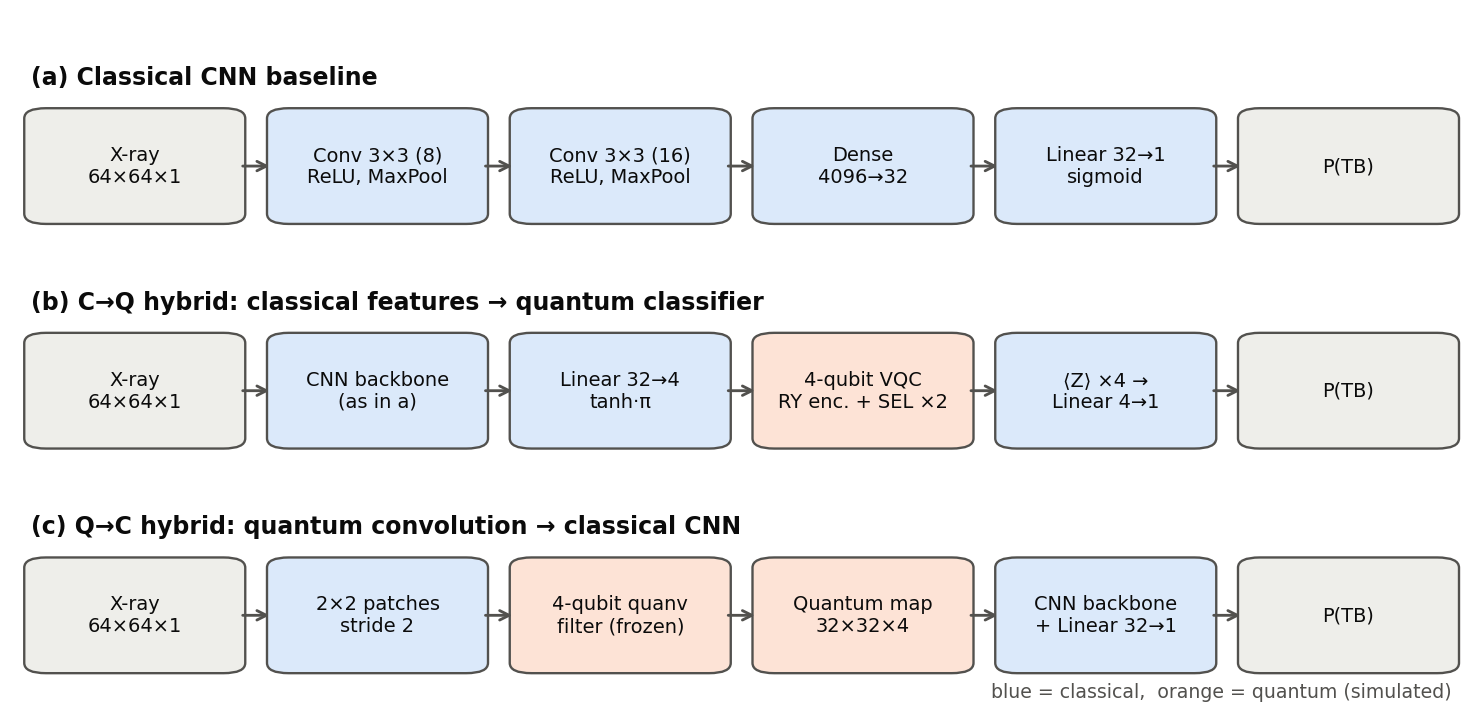
\includegraphics[width=\linewidth]{architectures.png}
  \caption{The three architectures: (a) classical CNN baseline,
  (b) classical-to-quantum hybrid, (c) quantum-to-classical hybrid. Blue
  blocks are classical, orange blocks are quantum.}
  \label{fig:architectures}
\end{figure}

\subsection{Classical CNN Baseline}
\label{sec:baseline}
The backbone has two blocks of $3 \times 3$ convolution (8 and 16 filters,
padding 1), ReLU~\cite{nair2010} and $2 \times 2$ max pooling, followed by
a dense projection of the $16 \times 16 \times 16$ feature map to 32 values
(131,104 parameters). The classical head is a linear layer with a sigmoid
(33 parameters). The model has 132,385 parameters in total; it is
deliberately small, so that the quantum component is not hidden behind a
very powerful classical network.

\subsection{Classical-to-Quantum (\cq) Hybrid}
\label{sec:cq}
The \cq{} hybrid replaces the linear head with a ``dressed'' variational
quantum classifier~\cite{mari2020}. A linear layer compresses the embedding
to $n = 4$ values $\mathbf{u}$, which are scaled to
$\mathbf{x} = \pi\tanh(\mathbf{u}) \in (-\pi, \pi)$ so that no two feature
values map to the same rotation, and encoded as
$\bigotimes_k R_Y(x_k)\ket{0}$. Two StronglyEntanglingLayers follow; each
applies $\mathrm{Rot}(\phi,\theta,\omega)$ to every qubit and a ring of
CNOTs of range 1 (first layer) and 2 (second layer), giving a weight tensor
of shape $(L, n, 3)$, i.e.\ 24 parameters. The four expectation values
$\expval{Z_k}$ (Eq.~\ref{eq:expz}) pass through a linear layer and a sigmoid
(Figure~\ref{fig:circuit_cq}). The head has 161 parameters and the whole
model 132,513, only 128 more than the baseline. The circuit is simulated with
PennyLane's \texttt{default.qubit} simulator inside a
\texttt{qml.qnn.TorchLayer}, so it trains like any PyTorch layer.

\begin{figure}[htbp]
  \centering
  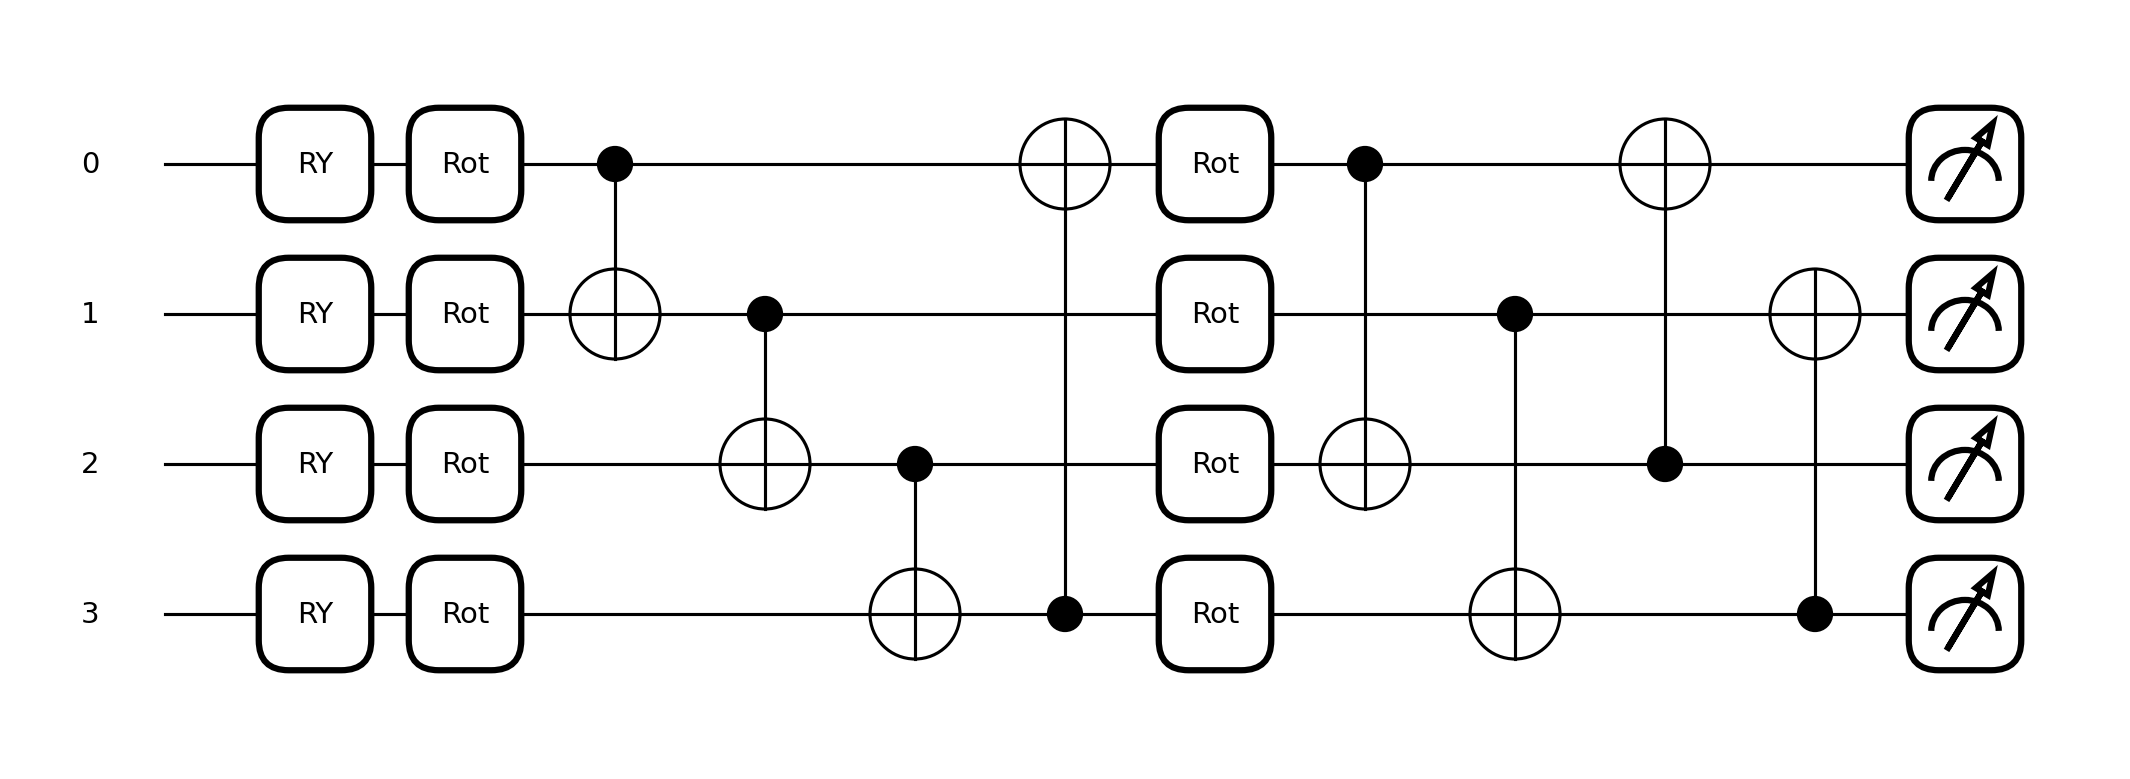
\includegraphics[width=0.85\linewidth]{circuit_cq_strong.png}
  \caption{Quantum circuit of the \cq{} head (4 qubits, depth 2): $R_Y$
  encoding, two StronglyEntanglingLayers, and measurement of $\expval{Z}$ on
  every qubit.}
  \label{fig:circuit_cq}
\end{figure}

For the ablation the head can use depth $L \in \{1,2,3,4\}$, $n \in
\{2,4,6,8\}$ qubits, amplitude encoding (the compression layer then outputs
$2^n$ values), BasicEntanglerLayers (one $R_X$ per qubit and a
nearest-neighbour CNOT ring), or no entanglement (the same rotations without
CNOTs, equivalent to four independent one-qubit models).

\subsection{Quantum-to-Classical (\qc) Hybrid}
\label{sec:qc}
The \qc{} hybrid places a quantum circuit at the start of the network as a
convolution filter~\cite{henderson2020}. The image is divided into 1,024
non-overlapping $2 \times 2$ patches; each pixel $p_k \in [0,1]$ is encoded
as $R_Y(\pi p_k)$, a fixed random circuit (one PennyLane \texttt{RandomLayers}
layer, seed 0, Figure~\ref{fig:circuit_quanv}) is applied, and the four
$\expval{Z_k}$ become four output channels. The resulting $4 \times 32
\times 32$ quantum feature map (Figure~\ref{fig:quanvmaps}) is processed by
the same CNN with four input channels. Because the input is half the size,
the model has only 34,297 parameters. As in the original method the filter
is random and frozen, so the transform is computed once for all 4,200 images
(4.3 million four-qubit circuits) and cached.

\begin{figure}[htbp]
  \centering
  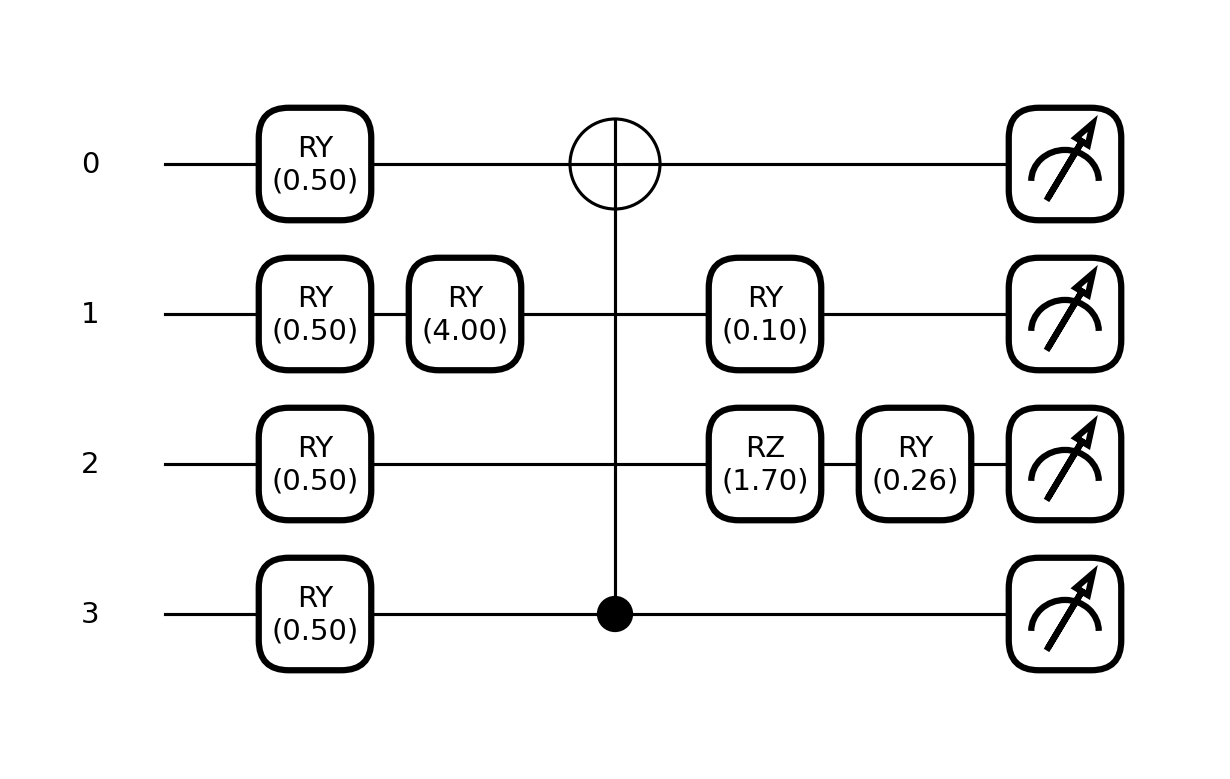
\includegraphics[width=0.5\linewidth]{circuit_quanv.png}
  \caption{The quanvolution filter for one $2\times2$ patch (encoding angles
  set to 0.5 for display). Its gates are drawn once from a fixed seed and not
  trained.}
  \label{fig:circuit_quanv}
\end{figure}

\begin{figure}[htbp]
  \centering
  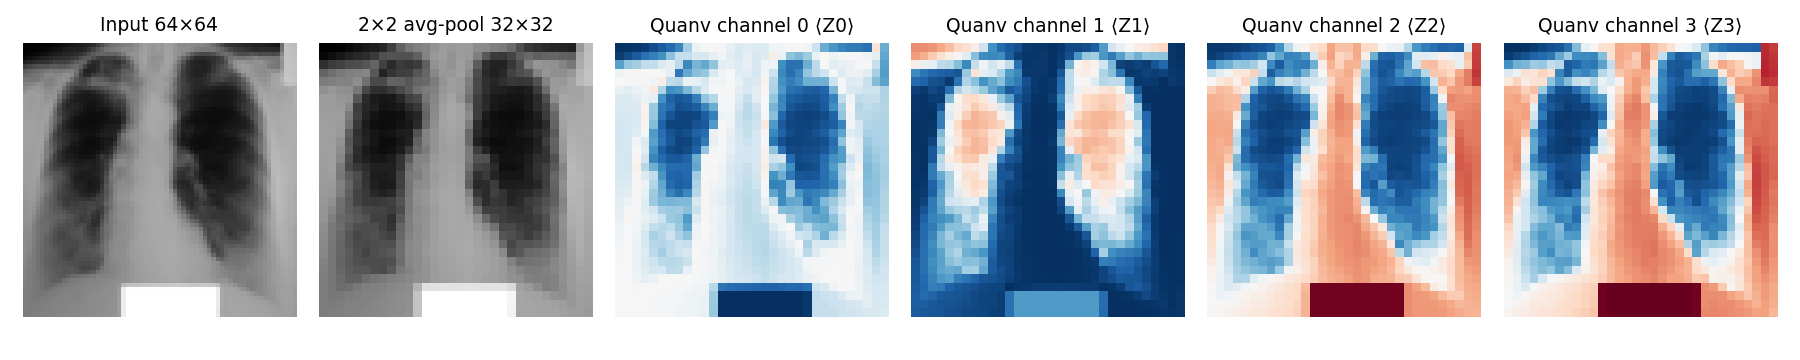
\includegraphics[width=\linewidth]{quanv_feature_maps.png}
  \caption{A TB radiograph at $64\times64$, its $2\times2$ average-pooled
  version, and the four channels of its quanvolution feature map. The
  rectangle at the bottom is a marker burned into the image, not anatomy.}
  \label{fig:quanvmaps}
\end{figure}

\subsection{Classical Control Models}
\label{sec:controls}
A hybrid that beats a baseline does not prove that its circuit is useful,
because it also differs in structure. Each hybrid is therefore paired with
classical models that differ from it only in the quantum component
(Table~\ref{tab:controls}). The matched head mirrors the quantum head step
for step, so any difference can only come from \emph{what} the four-to-four
transformation computes. The three \qc{} controls separate three
explanations: any fixed non-linear patch map, the downsampling itself, and
a patch filter that is allowed to learn.

\begin{table}[htbp]
\centering
\footnotesize
\caption{Models in the main study and what each one controls for.}
\label{tab:controls}
\begin{tabular}{p{4.2cm}rp{7.2cm}}
\toprule
Model & Params & Purpose \\
\midrule
Classical CNN & 132,385 & Baseline. \\
CNN + matched classical head & 132,509 & Control for \cq: the circuit is
replaced by a classical $\mathrm{Linear}(4,4)$ and $\tanh$ (157 head
parameters versus 161). \\
\cq{} hybrid & 132,513 & CNN + variational quantum head. \\
\midrule
\qc{} hybrid & 34,297 & Quanvolution + CNN. \\
Random patch + CNN & 34,297 & Control for \qc: fixed random classical map
$\tanh(W\pi\mathbf{p} + \mathbf{b})$ with the same input and output. \\
Avg-pool + CNN & 34,081 & Control for \qc: plain $2\times2$ average pooling. \\
Learned $2\times2$ conv + CNN & 34,317 & Control for \qc: trainable
$2\times2$, stride-2 convolution with four channels and $\tanh$. \\
\bottomrule
\end{tabular}
\end{table}

\subsection{Transfer Learning with ResNet18}
\label{sec:resnet}
To test the findings with a strong backbone, the small CNN is replaced by an
ImageNet-pretrained ResNet18~\cite{he2016}. The grayscale channel is
repeated three times, the ImageNet classifier is replaced by a linear layer
to the same 32-dimensional embedding, so either head can be attached, and
the pretrained layers are fine-tuned with a ten times smaller learning rate
($10^{-4}$). The resulting models have about 11.19 million parameters.

\section{Training and Evaluation Protocol}
\label{sec:training}
All models are trained identically: binary cross-entropy
(Eq.~\ref{eq:bce}), Adam~\cite{kingma2015} with learning rate $10^{-3}$,
batch size 32 and 15 epochs on a CPU, with no per-model tuning. In the main
study every run keeps the weights of the epoch with the lowest validation
loss, and runs on 2--10\% of the data train for 40 epochs, since 15 epochs
on 58 images are only about 30 gradient steps. Quantum gradients are
computed by backpropagation through the simulator; on hardware the
parameter-shift rule (Eq.~\ref{eq:pshift}) would be used, and we verify that
the two agree.

\label{sec:eval}
An image is predicted as TB when its probability is at least 0.5. With TB as
the positive class we report
\begin{align}
\mathrm{Accuracy} &= \frac{TP + TN}{TP + TN + FP + FN}, &
\mathrm{Recall} &= \frac{TP}{TP + FN}, \\
F_1 &= \frac{2\cdot\mathrm{Precision}\cdot\mathrm{Recall}}{\mathrm{Precision}+\mathrm{Recall}}, &
\mathrm{Precision} &= \frac{TP}{TP + FP},
\end{align}
and the ROC-AUC, the probability that
a random TB image is scored above a random normal image~\cite{fawcett2006}.
Recall matters most clinically, since a missed TB case is more harmful than
a false alarm. Multi-seed experiments report mean $\pm$ standard deviation
over seeds 42, 43 and 44, and any ``best'' configuration is chosen on
validation F1, never on the test set.

Because all models are scored on the same test images, two models are
compared image by image with McNemar's exact test~\cite{mcnemar1947}. If $b$
images are classified correctly by model A only and $c$ by model B only, then
under the null hypothesis of equal error rates
$b \sim \mathrm{Binomial}(b + c, \tfrac{1}{2})$. The test is run separately
for each seed, and $p < 0.05$ is treated as significant.

\label{sec:qa_protocol}
The circuits are also characterised directly: expressibility and entangling
capability of the trainable block (three entanglement patterns, depths 1--4,
5,000 random parameter pairs); the variance over 500 random initialisations
of the gradient of a local cost $\expval{Z_0}$ and a global cost
$\expval{Z^{\otimes n}}$ for 2 to 10 qubits at depths 2 and 10; the trained
\cq{} model (seed 42) re-evaluated with 10 to 10,000 measurement shots and
with depolarising noise (Eq.~\ref{eq:depol}) after every layer for $p$ up to
0.2, with its weights fixed; and a comparison of parameter-shift and
backpropagation gradients of the trained circuit.

\chapter{Experimental Setup and Results Analysis}
\label{ch:results}

\section{Experimental Setup}
\label{sec:env}
All experiments ran on one laptop with an AMD Ryzen 7 6800H CPU (8 cores),
15.3 GB of memory and no GPU, under Windows 11 with Python 3.10.11, PyTorch
2.14.1, PennyLane 0.42.3, scikit-learn~\cite{pedregosa2011} 1.7.2 and NumPy
2.2.6. Circuits were simulated exactly with \texttt{default.qubit}, except
in the noise experiments, which used finite shots and the
\texttt{default.mixed} density-matrix simulator. Each experiment is a
separate script that writes its configuration and metrics to
\texttt{results/tb/}. Because the laptop was shared, training times varied
between runs and are given as rough indications only. All results refer to
the same 630 test images (525 normal, 105 TB).

In a first single-seed run (seed 42), replacing the 33-parameter linear head
with the 161-parameter quantum head raised accuracy from 97.46\% to 98.41\%
(16 errors against 10; missed TB cases 9 against 7) at about three times the
training time. Since the two models differ in more than the circuit, the
following experiments use repeated seeds and matched controls.

\section{Circuit Design Ablation}
\label{sec:res_ablation}
The ablation varies one property of the \cq{} circuit at a time, starting
from 4 qubits, depth 2, angle encoding and strong entanglement (seed 42).
Figure~\ref{fig:ablation} shows all twelve configurations on a common axis.

\begin{figure}[htbp]
  \centering
  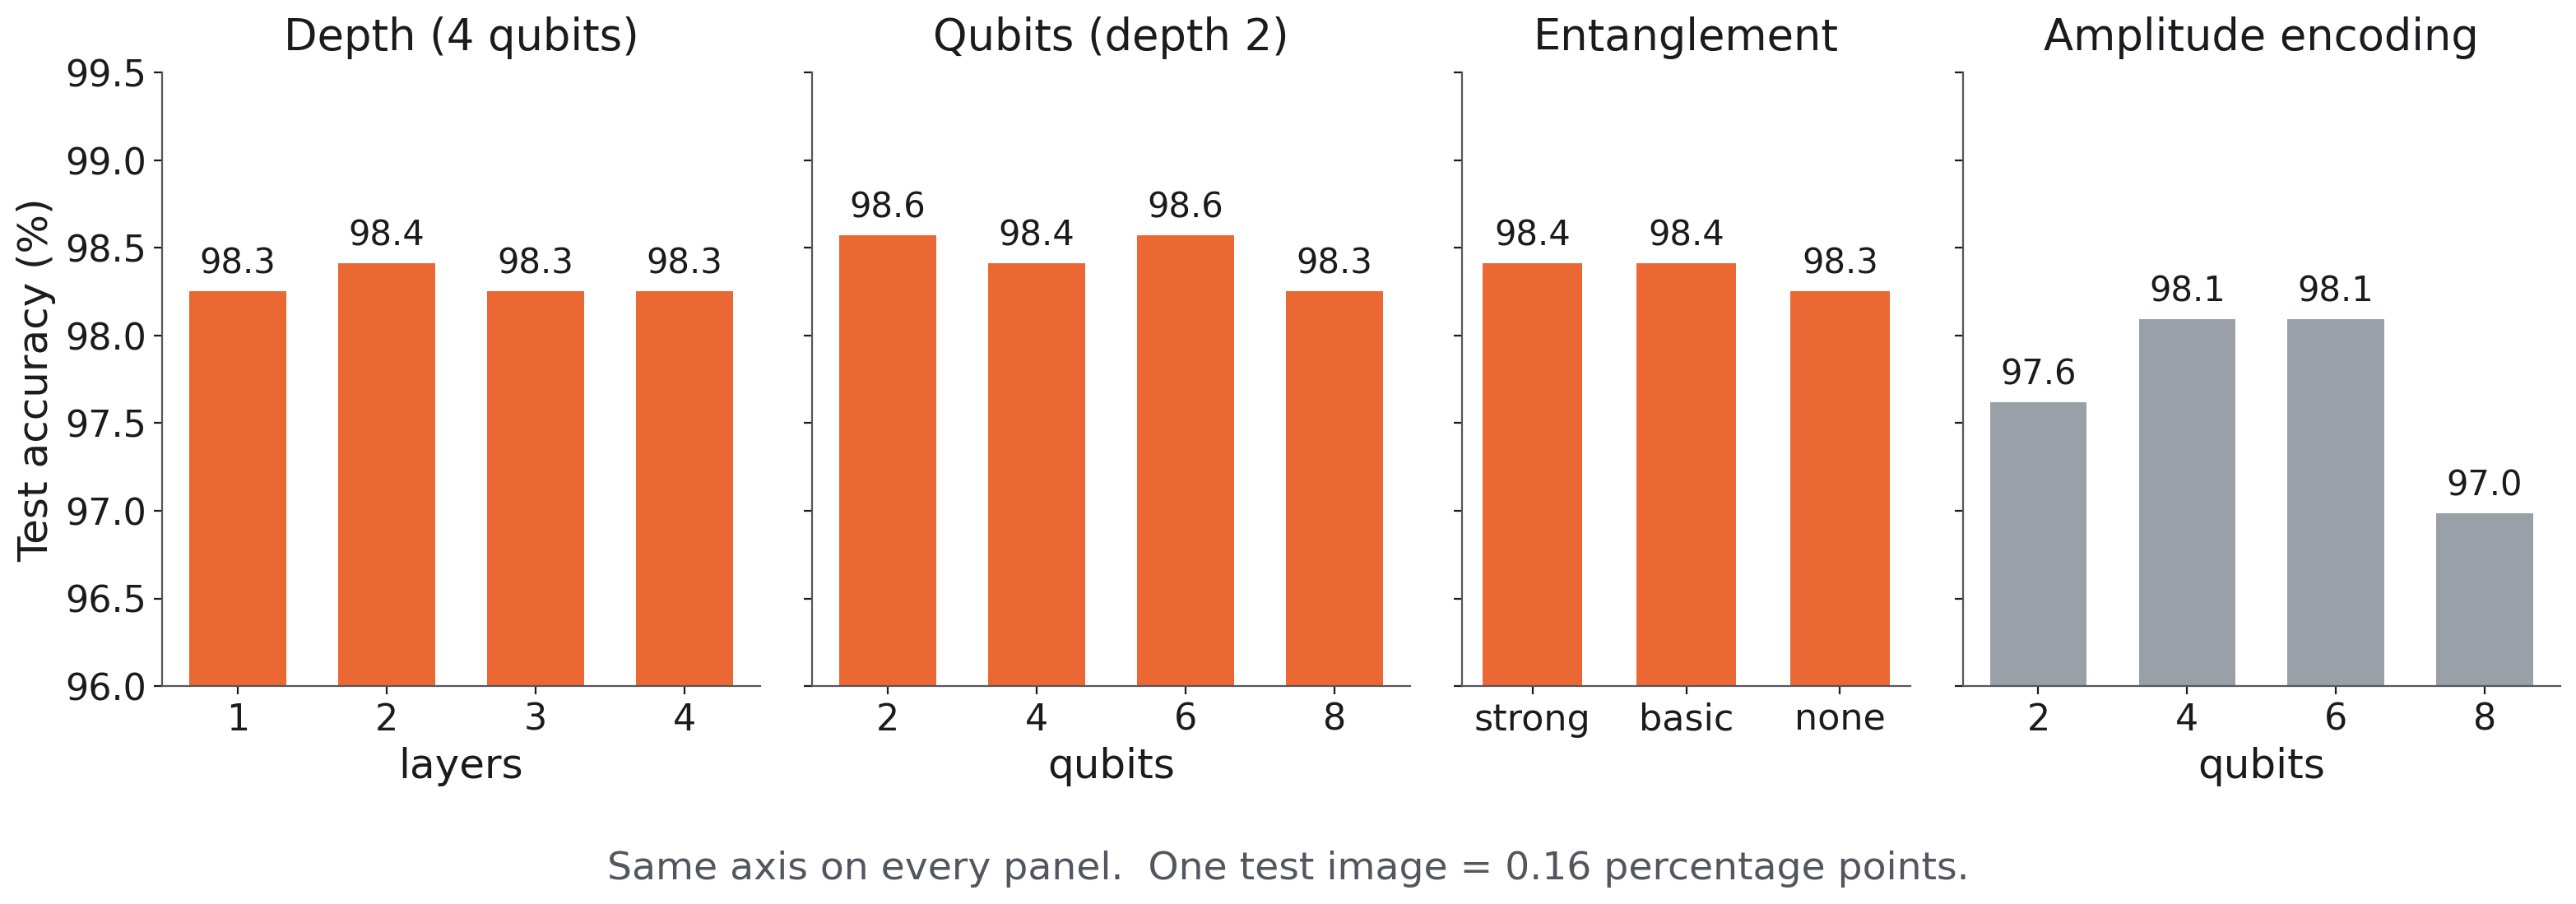
\includegraphics[width=\linewidth]{ablation_summary.png}
  \caption{Test accuracy of all twelve circuit configurations of the \cq{}
  hybrid (seed 42). All panels share one axis; one test image corresponds to
  0.16 percentage points.}
  \label{fig:ablation}
\end{figure}

Depth changed test accuracy only between 98.25\% and 98.41\%, one test
image, while training time grew roughly linearly with depth; the best
validation F1 was obtained at depth 1. Strong and basic entanglement gave
identical results (98.41\%, F1 0.9515), and removing entanglement cost a
single test image. With angle encoding, 2 to 8 qubits gave 98.25--98.57\%.
Amplitude encoding was worse in every case (96.98--98.10\%) and worst at 8
qubits, where 256 amplitudes must be produced from a 32-dimensional
embedding and normalisation discards the vector's length. Within the tested
range the circuit design therefore barely affects accuracy: after the CNN
has extracted its features, the four-to-one decision does not need the
extra correlations that entanglement provides. Angle encoding is
consistently preferable, and small circuits are as good as large ones.

\section{Backbone and Head Comparison}
\label{sec:res_backbone}
The third experiment crosses two backbones with two heads, each with three
seeds (Table~\ref{tab:comparison}).

\begin{table}[htbp]
\centering
\footnotesize
\caption{Backbone $\times$ head comparison: mean $\pm$ standard deviation over seeds 42, 43 and 44 on the fixed test set.}
\label{tab:comparison}
\begin{adjustbox}{max width=\linewidth}
\begin{tabular}{lrrrrrrr}
\toprule
Model & Params & Accuracy (\%) & Precision & Recall & F1 & ROC-AUC & Time (s) \\
\midrule
CNN + classical & 132,385 & 98.04 $\pm$ 0.56 & 0.9326 $\pm$ 0.0286 & 0.9524 $\pm$ 0.0381 & 0.9418 $\pm$ 0.0172 & 0.9975 $\pm$ 0.0004 & 16 \\
CNN + quantum & 132,513 & 98.41 $\pm$ 0.32 & 0.9612 $\pm$ 0.0094 & 0.9429 $\pm$ 0.0165 & 0.9519 $\pm$ 0.0098 & 0.9980 $\pm$ 0.0014 & 46 \\
ResNet18 + classical & 11,192,961 & 99.21 $\pm$ 0.57 & 0.9875 $\pm$ 0.0216 & 0.9651 $\pm$ 0.0361 & 0.9758 $\pm$ 0.0178 & 0.9991 $\pm$ 0.0006 & 314 \\
ResNet18 + quantum & 11,193,089 & 99.47 $\pm$ 0.18 & 0.9936 $\pm$ 0.0056 & 0.9746 $\pm$ 0.0145 & 0.9839 $\pm$ 0.0057 & 0.9961 $\pm$ 0.0046 & 346 \\
\bottomrule
\end{tabular}
\end{adjustbox}
\end{table}


With both backbones the quantum head gave a higher mean accuracy and F1 and
a smaller standard deviation: $98.41 \pm 0.32\%$ against $98.04 \pm 0.56\%$
for the small CNN, and $99.47 \pm 0.18\%$ against $99.21 \pm 0.57\%$ for
ResNet18. The backbone mattered about three times more than the head:
ResNet18 raised accuracy by about one percentage point, at the cost of 85
times more parameters and about 20 times longer training. ROC-AUC exceeded
0.996 for every model, so all four rank images almost perfectly and the
differences lie in where the 0.5 threshold falls. The head differences are
comparable to the seed-to-seed variation and are tested for significance
next.

\section{Main Study: Hybrids versus Matched Controls}
\label{sec:res_study}
The main experiment trains the seven models of Table~\ref{tab:controls}
with three seeds on five training-set sizes (105 runs).
Table~\ref{tab:study_full} gives the full-data results and
Table~\ref{tab:mcnemar} the paired tests.

\begin{table}[htbp]
\centering
\footnotesize
\caption{Main study on the full training set (2,940 images): mean $\pm$ std over three seeds. Head parameters count only the classifier head.}
\label{tab:study_full}
\begin{adjustbox}{max width=\linewidth}
\begin{tabular}{lrrrrrrr}
\toprule
Model & Params & Head & Accuracy (\%) & Recall & F1 & ROC-AUC & Time (s) \\
\midrule
Classical CNN & 132,385 & 33 & 97.67 $\pm$ 0.33 & 0.9238 $\pm$ 0.0095 & 0.9298 $\pm$ 0.0094 & 0.9966 $\pm$ 0.0009 & 15 \\
CNN + matched classical head & 132,509 & 157 & 97.72 $\pm$ 0.40 & 0.9079 $\pm$ 0.0145 & 0.9301 $\pm$ 0.0119 & 0.9959 $\pm$ 0.0011 & 17 \\
C$\rightarrow$Q hybrid (CNN + quantum head) & 132,513 & 161 & 98.41 $\pm$ 0.32 & 0.9429 $\pm$ 0.0165 & 0.9519 $\pm$ 0.0098 & 0.9980 $\pm$ 0.0014 & 43 \\
Q$\rightarrow$C hybrid (quanvolution + CNN) & 34,297 & 33 & 97.88 $\pm$ 0.33 & 0.9270 $\pm$ 0.0145 & 0.9359 $\pm$ 0.0096 & 0.9954 $\pm$ 0.0017 & 5 \\
Random patch + CNN (control) & 34,297 & 33 & 90.53 $\pm$ 0.87 & 0.5206 $\pm$ 0.0715 & 0.6449 $\pm$ 0.0543 & 0.9336 $\pm$ 0.0035 & 4 \\
Avg-pool + CNN (control) & 34,081 & 33 & 98.15 $\pm$ 0.09 & 0.9556 $\pm$ 0.0110 & 0.9451 $\pm$ 0.0020 & 0.9956 $\pm$ 0.0008 & 4 \\
Learned 2x2 conv + CNN (control) & 34,317 & 33 & 98.31 $\pm$ 0.72 & 0.9524 $\pm$ 0.0000 & 0.9497 $\pm$ 0.0204 & 0.9956 $\pm$ 0.0033 & 7 \\
\bottomrule
\end{tabular}
\end{adjustbox}
\end{table}

\begin{table}[htbp]
\centering
\scriptsize
\caption{McNemar exact test between each hybrid and a classical comparator on the full-data runs. Each cell gives the p-value and, in brackets, the number of test images only the hybrid got right / only the comparator got right.}
\label{tab:mcnemar}
\begin{adjustbox}{max width=\linewidth}
\begin{tabular}{llrrr}
\toprule
Hybrid & Compared with & Seed 42 & Seed 43 & Seed 44 \\
\midrule
C$\rightarrow$Q hybrid (CNN + quantum head) & CNN + matched classical head & 0.092 (10/3) & 0.146 (9/3) & 1.000 (7/7) \\
Q$\rightarrow$C hybrid (quanvolution + CNN) & Random patch + CNN (control) & $<$0.001 (57/2) & $<$0.001 (49/7) & $<$0.001 (50/8) \\
Q$\rightarrow$C hybrid (quanvolution + CNN) & Avg-pool + CNN (control) & 1.000 (5/4) & 0.344 (3/7) & 0.791 (6/8) \\
Q$\rightarrow$C hybrid (quanvolution + CNN) & Learned 2x2 conv + CNN (control) & 1.000 (4/4) & 1.000 (6/6) & 0.057 (3/11) \\
C$\rightarrow$Q hybrid (CNN + quantum head) & Classical CNN & 0.424 (9/5) & 0.227 (8/3) & 0.267 (9/4) \\
Q$\rightarrow$C hybrid (quanvolution + CNN) & Classical CNN & 0.453 (5/2) & 0.804 (7/9) & 0.581 (8/5) \\
\bottomrule
\end{tabular}
\end{adjustbox}
\end{table}


\paragraph{Does the quantum head help?} The \cq{} hybrid was the best
small-CNN model ($98.41 \pm 0.32\%$, F1 $0.952 \pm 0.010$). Its matched
classical control, with the same bottleneck, scored $97.72 \pm 0.40\%$ and
$0.930 \pm 0.012$, almost exactly like the plain CNN ($97.67 \pm 0.33\%$,
$0.930 \pm 0.009$), so the bottleneck alone does not explain the gain, and
the hybrid was ahead for every seed. The McNemar tests, however, are not
significant: $p$ = 0.092, 0.146 and 1.000 against the matched head and
0.424, 0.227 and 0.267 against the CNN. With error rates around 2\%, two
models disagree on only a handful of the 630 images, too few to rule out
chance. The quantum head thus gives a small, consistent improvement of
about 0.7 percentage points that this dataset cannot confirm statistically.

\paragraph{Does the quantum filter help?} The \qc{} hybrid reached
$97.88 \pm 0.33\%$ with 34,297 parameters, indistinguishable from the
132,385-parameter CNN ($p$ = 0.453, 0.804, 0.581). It was far better than
the random classical patch map ($90.53\%$, $p < 0.001$ for every seed),
whose $\tanh$ saturates and turns patches into nearly binary values, while
the quantum filter's cosine-shaped response keeps the detail. But
$2\times2$ average pooling ($98.15 \pm 0.09\%$) and a learned $2\times2$
convolution ($98.31 \pm 0.72\%$) did as well as the quantum filter
($p \geq 0.057$). The four-fold parameter saving therefore comes from
halving the resolution, not from the quantum computation, mirroring the
finding of Henderson et al.~\cite{henderson2020}.

\paragraph{Low-data regime.} Table~\ref{tab:study_lowdata} gives F1 for
smaller training sets. With 2\% of the data (58 images), the \qc{} hybrid
and average pooling had the highest F1 (0.677 and 0.666), and the \qc{}
hybrid was by far the most stable model (standard deviation 0.020). The
four-dimensional bottleneck heads were unreliable with little data: the
matched classical head predicted ``Normal'' for every test image in all
three seeds at 2\% and in two of three seeds at 5\% and 25\%, and the \cq{}
hybrid reached only $0.341 \pm 0.250$ at 2\%. This is a calibration failure
rather than a failure to learn: at 2\% the \cq{} hybrid had the
\emph{highest} ROC-AUC of all models (0.927 against 0.911 for the CNN), so it
ranks images well but its probabilities do not cross the 0.5 threshold in
the right places. From 5\% upwards the classical CNN had the highest or
joint-highest F1, and only with the full data did the \cq{} hybrid move
ahead. The experiment therefore does not support a general claim that the
hybrids learn more from fewer examples.

\begin{table}[htbp]
\centering
\scriptsize
\caption{Test F1 (mean $\pm$ std, three seeds) versus the fraction of the training split used. Validation and test sets are never reduced.}
\label{tab:study_lowdata}
\begin{adjustbox}{max width=\linewidth}
\begin{tabular}{lrrrrr}
\toprule
Model & 2\% (58) & 5\% (147) & 10\% (294) & 25\% (735) & 100\% (2940) \\
\midrule
Classical CNN & 0.601 $\pm$ 0.170 & 0.815 $\pm$ 0.027 & 0.880 $\pm$ 0.009 & 0.909 $\pm$ 0.008 & 0.930 $\pm$ 0.009 \\
CNN + matched classical head & 0.000 $\pm$ 0.000 & 0.263 $\pm$ 0.455 & 0.876 $\pm$ 0.010 & 0.309 $\pm$ 0.535 & 0.930 $\pm$ 0.012 \\
C$\rightarrow$Q hybrid (CNN + quantum head) & 0.341 $\pm$ 0.250 & 0.787 $\pm$ 0.064 & 0.850 $\pm$ 0.077 & 0.871 $\pm$ 0.080 & 0.952 $\pm$ 0.010 \\
Q$\rightarrow$C hybrid (quanvolution + CNN) & 0.677 $\pm$ 0.020 & 0.754 $\pm$ 0.093 & 0.834 $\pm$ 0.028 & 0.884 $\pm$ 0.015 & 0.936 $\pm$ 0.010 \\
Random patch + CNN (control) & 0.000 $\pm$ 0.000 & 0.416 $\pm$ 0.086 & 0.456 $\pm$ 0.065 & 0.490 $\pm$ 0.052 & 0.645 $\pm$ 0.054 \\
Avg-pool + CNN (control) & 0.666 $\pm$ 0.138 & 0.749 $\pm$ 0.099 & 0.862 $\pm$ 0.020 & 0.892 $\pm$ 0.011 & 0.945 $\pm$ 0.002 \\
Learned 2x2 conv + CNN (control) & 0.451 $\pm$ 0.076 & 0.705 $\pm$ 0.155 & 0.768 $\pm$ 0.092 & 0.857 $\pm$ 0.075 & 0.950 $\pm$ 0.020 \\
\bottomrule
\end{tabular}
\end{adjustbox}
\end{table}


\section{Quantum Circuit Analysis}
\label{sec:res_expr}
Figure~\ref{fig:expr} characterises the trainable block of the \cq{}
circuit without any data. With entangling gates, expressibility improves
sharply from depth 1 to depth 2 (KL divergence 0.308 to 0.0083 for strong
entanglement) and reaches 0.004--0.005 at depth 3, close to Haar-random.
Without entanglement it stays at 0.19--0.30 whatever the depth, because
product states can never cover the four-qubit state space. The entangling
capability of the strong and basic patterns is 0.79--0.87, close to the
Haar-random value $14/17 \approx 0.82$, and exactly zero without
entanglement. Read together with the ablation, the circuits differ strongly
as quantum objects --- at depths 2 to 4 the no-entanglement circuit is 20 to
60 times less expressive --- yet give almost the same accuracy: the task, as
posed after a classical feature extractor, does not use the extra capacity.

\begin{figure}[htbp]
  \centering
  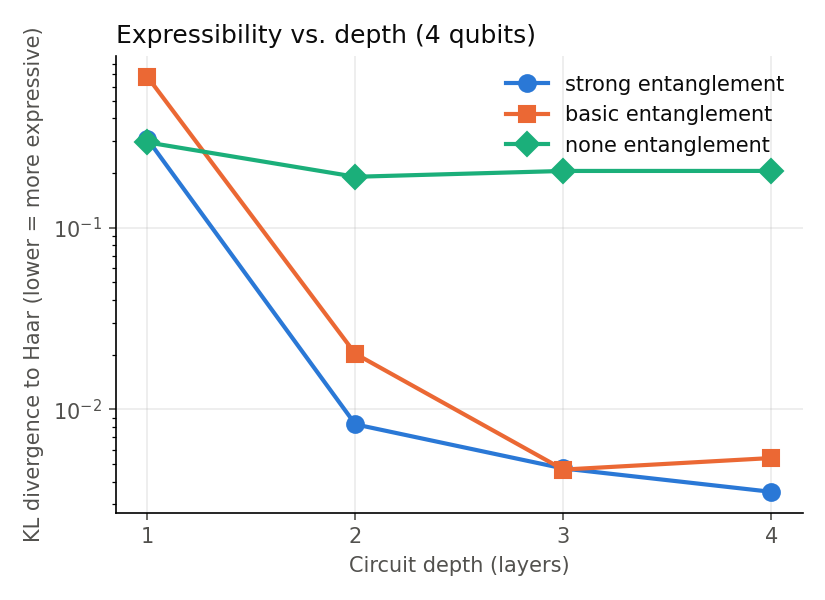
\includegraphics[width=0.48\linewidth]{expressibility.png}\hfill
  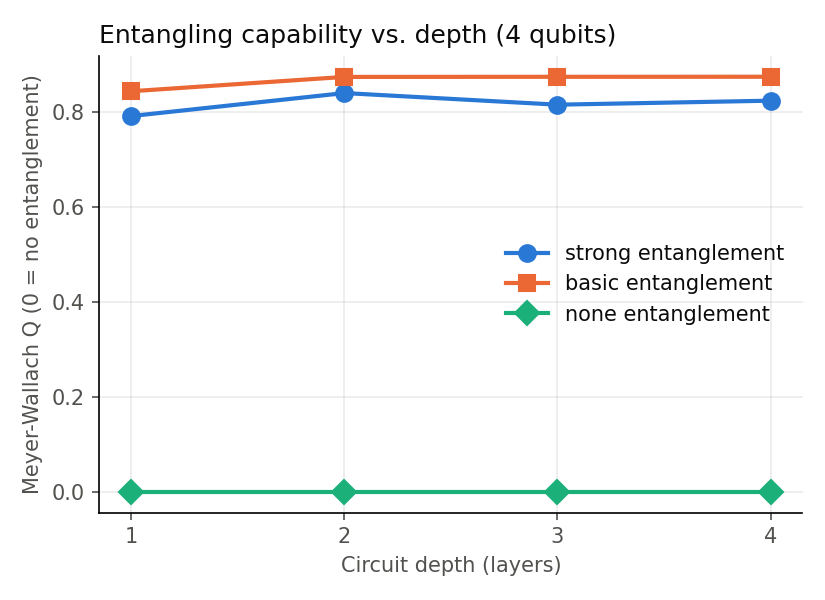
\includegraphics[width=0.48\linewidth]{entangling_capability.png}
  \caption{Expressibility (left, lower is more expressive) and entangling
  capability (right) of the three entanglement patterns versus depth,
  4 qubits.}
  \label{fig:expr}
\end{figure}

\label{sec:res_bp}
Figure~\ref{fig:bp} shows how the gradient variance scales with the number
of qubits. For depth 10 it falls from 0.150 at 2 qubits to
$4.2 \times 10^{-4}$ at 10 qubits for the local cost, and from 0.122 to
$5.0 \times 10^{-4}$ for the global cost --- about a factor of two per added
qubit, the $2^{-n}$ decay predicted by McClean et al.~\cite{mcclean2018}. The
depth-2 curves follow the same trend but are noisier, and we did not observe
the advantage of local over global costs reported by Cerezo et
al.~\cite{cerezo2021}, possibly because the long-range CNOTs spread
information across all qubits even at depth 2. At 4 qubits the variance is
60 to 300 times larger than at 10, which supports the choice of a small
circuit, particularly for hardware, where each gradient must be estimated
from finite shots.

\begin{figure}[htbp]
  \centering
  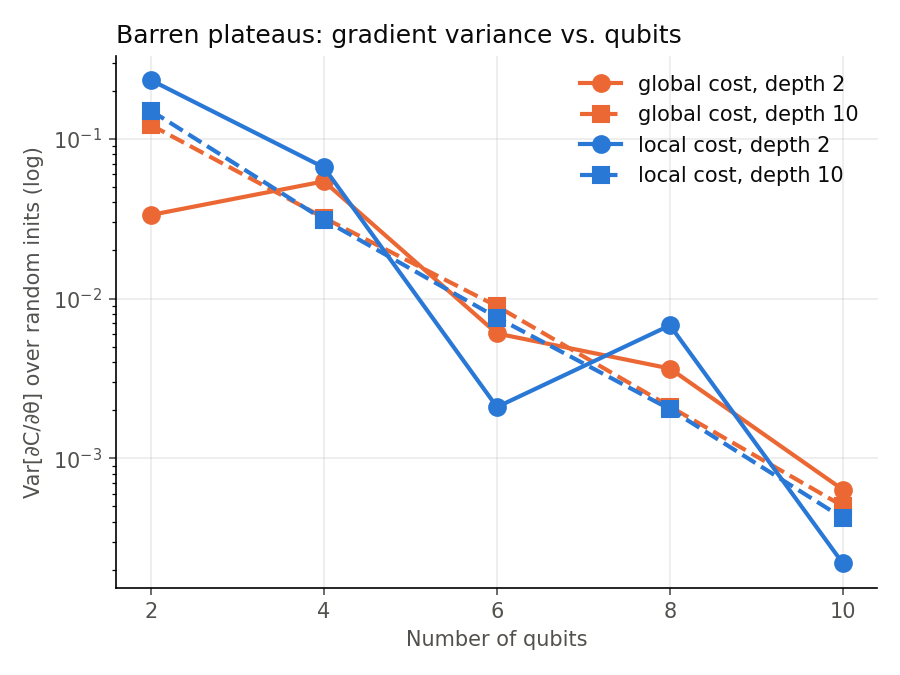
\includegraphics[width=0.6\linewidth]{barren_plateaus.png}
  \caption{Variance of the cost gradient over 500 random initialisations
  versus number of qubits for local and global costs at depths 2 and 10.}
  \label{fig:bp}
\end{figure}

\section{Robustness to Shot Noise and Hardware Noise}
\label{sec:res_noise}
Figure~\ref{fig:noise} shows the trained \cq{} model (seed 42) evaluated as
on an imperfect device. With only 10 shots per expectation value, which gives
each $\expval{Z_k}$ a standard error of up to 0.32, accuracy was 98.25\%
against 98.41\% for exact values, and with 50 to 10,000 shots it stayed
within 98.25--98.57\%. With depolarising noise after every layer it stayed
within 98.41--98.57\% up to $p = 0.2$, and the AUC was unchanged at 0.9987.
Most test images lie far from the decision boundary, and depolarisation
shrinks all four outputs by a similar factor (about 0.65--0.75 at $p = 0.1$),
so the direction of the output vector and the ranking of images are
preserved. Finally, parameter-shift and backpropagation gradients of the
trained circuit agreed to $1.1 \times 10^{-15}$, so the model could be
trained on hardware without any change. These results apply to small,
shallow circuits; deeper circuits or less uniform noise would degrade more.

\begin{figure}[htbp]
  \centering
  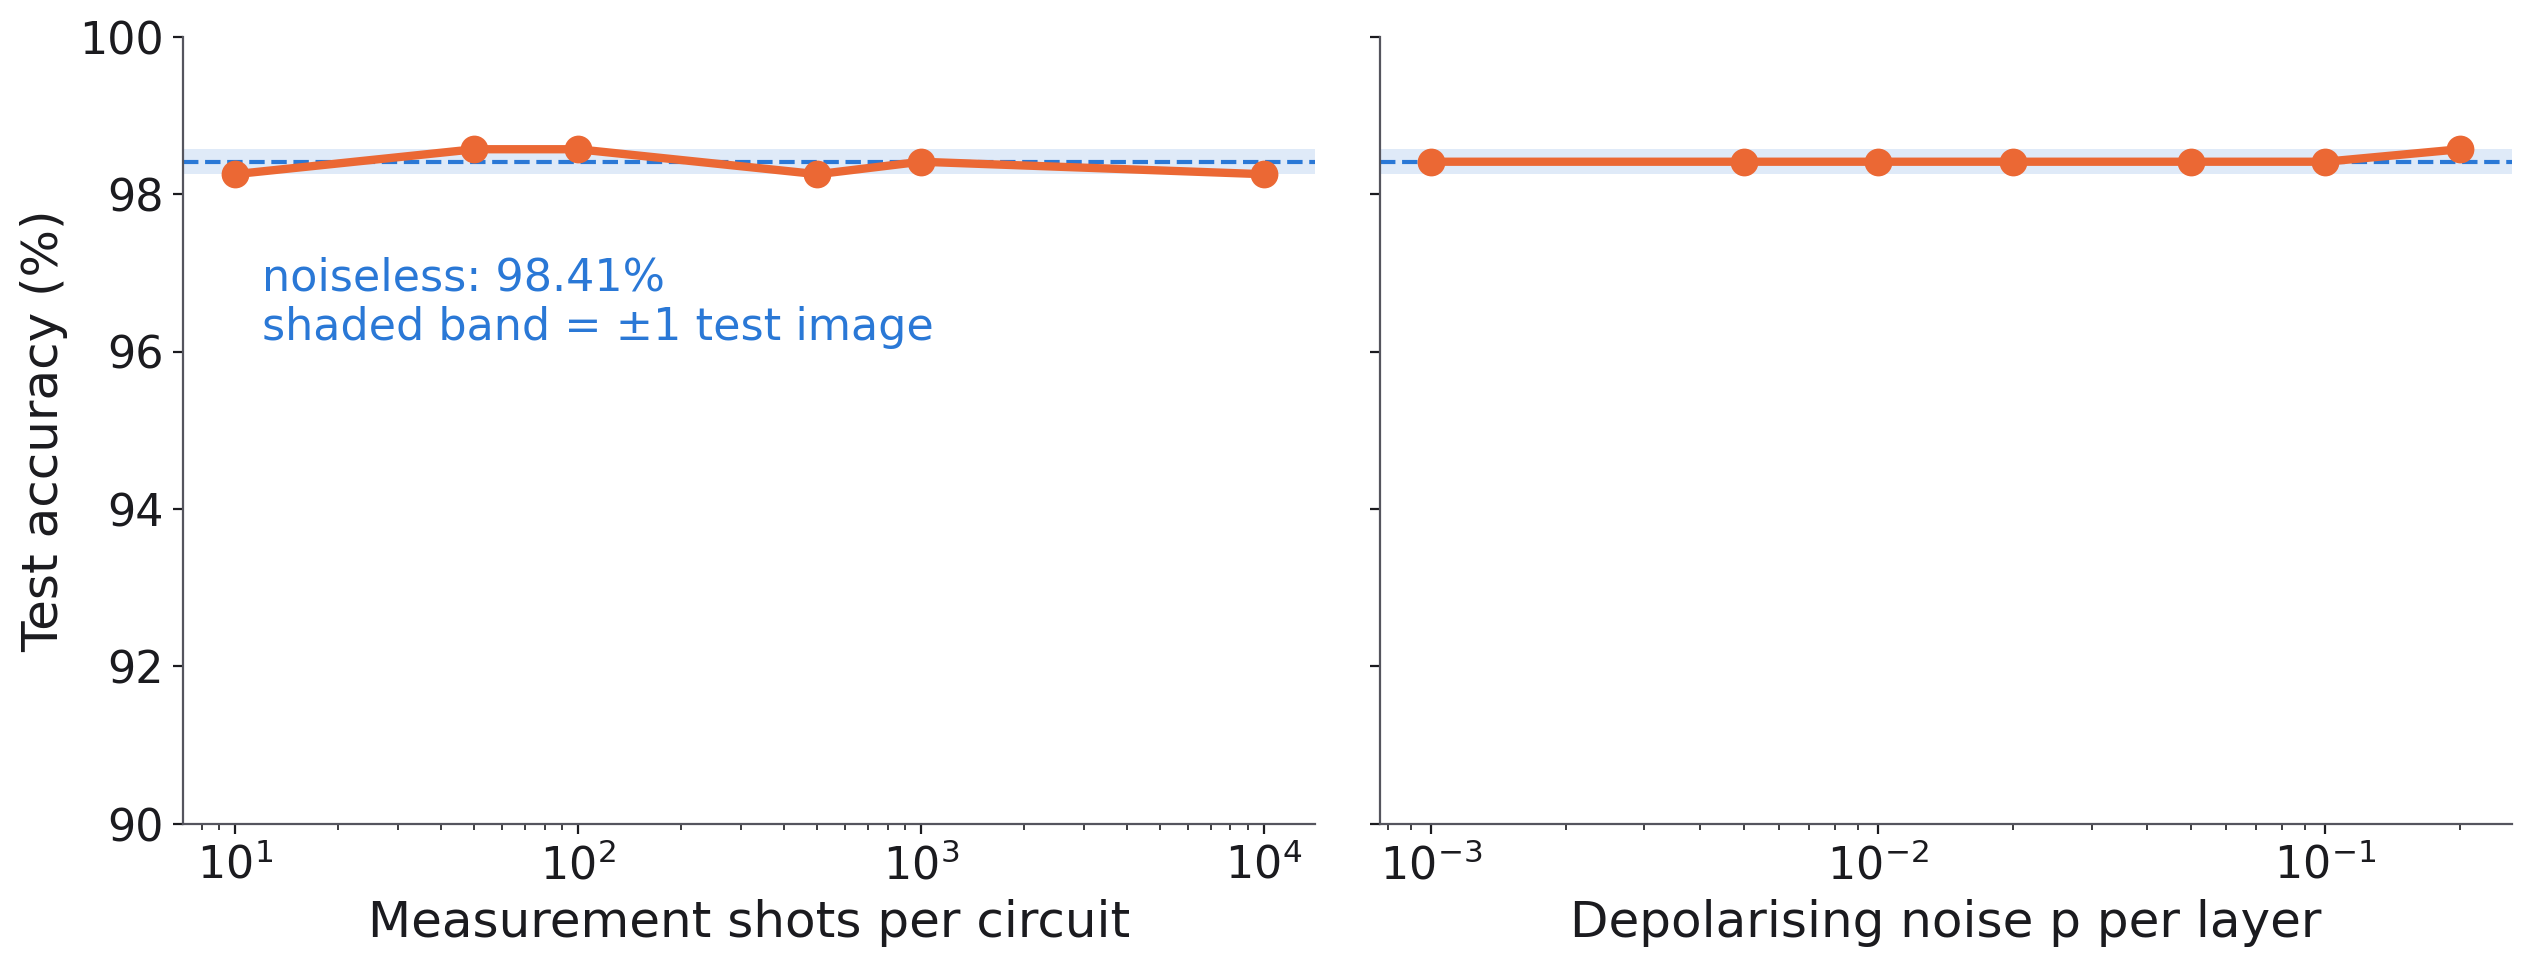
\includegraphics[width=\linewidth]{nisq_robustness.png}
  \caption{Test accuracy of the trained \cq{} model versus measurement shots
  (left) and depolarising probability per layer (right). The shaded band is
  $\pm 1$ test image around the noiseless accuracy.}
  \label{fig:noise}
\end{figure}

\section{Error Analysis}
\label{sec:res_errors}
For seed 42, only 22 of the 630 test images were misclassified by any of the
four backbone $\times$ head models, and a single image by all four. The
small-CNN models' errors were dominated by missed TB cases (9 of 16 for the
classical head, 7 of 10 for the quantum head), the more harmful error in
screening, while ResNet18 reduced the errors to one or two.
Figure~\ref{fig:errors} shows the most confident mistakes of the CNN with a
quantum head. They include TB cases with subtle changes that are hard to see
at $64 \times 64$ pixels and a normal portable film with text markers, a
reminder that models may partly learn differences between image sources
rather than disease.

\begin{figure}[htbp]
  \centering
  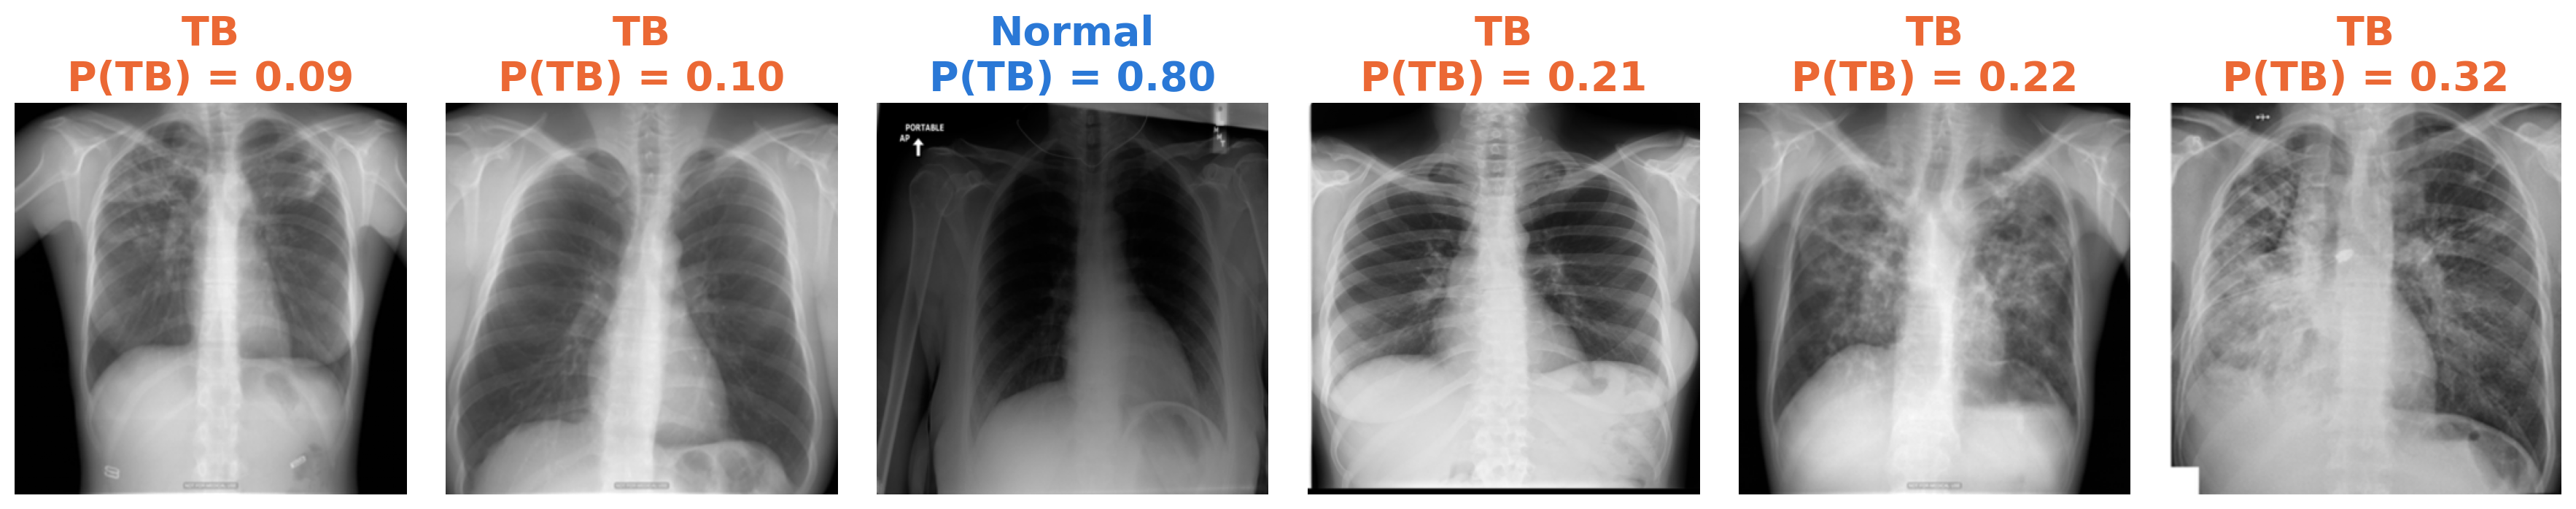
\includegraphics[width=\linewidth]{errors_labeled.png}
  \caption{The six most confident mistakes of the CNN + quantum head model
  (seed 42), with the true class and the predicted probability of TB.}
  \label{fig:errors}
\end{figure}

\section{Discussion}
\label{sec:discussion}
Rahman et al.~\cite{rahman2020} reported 98--99\% accuracy on the same
dataset with large pretrained CNNs on much larger images. Our classical CNN
(97.67\%), \cq{} hybrid (98.41\%) and ResNet18 with a quantum head
(99.47\%) fall in the same range, but the comparison is only indicative,
since splits, preprocessing and resolution differ and a 630-image test set
gives each accuracy an uncertainty of about $\pm 1$ percentage point.

Taken together, the experiments show that a quantum classifier head is a
viable drop-in replacement for a classical one, with a small, consistent but
not significant gain; that the quanvolution filter is a reasonable but not a
special feature extractor, whose efficiency comes from downsampling; that
circuit design changes expressibility by more than an order of magnitude but
accuracy by at most a test image or two; and that small hybrid circuits are
trainable and robust to the noise of current hardware. What the evidence
does \emph{not} show is a quantum advantage: no hybrid was significantly
better than its best classical counterpart, consistent with the expectation
that small, classically simulable circuits cannot outperform classical
models of similar size.

\chapter{Conclusion and Future Work}
\label{ch:conclusion}

\section{Conclusion}
This project built and evaluated hybrid quantum--classical neural networks
for detecting tuberculosis in chest radiographs, in two placements: a \cq{}
model in which a CNN's features are classified by a four-qubit variational
circuit, and a \qc{} model in which a four-qubit quanvolution filter
transforms image patches before a CNN. Each hybrid was compared with
classical controls of the same structure and size, with three seeds, five
training-set sizes and paired McNemar tests, and the circuits were analysed
directly. The main findings are:
\begin{enumerate}
  \item The \cq{} hybrid reached $98.41 \pm 0.32\%$ accuracy (F1
        $0.952 \pm 0.010$) against $97.72 \pm 0.40\%$ for a matched
        classical head and $97.67 \pm 0.33\%$ for the CNN; the gain was
        consistent across seeds but not significant ($p = 0.09$--$1.00$).
        With ResNet18 the quantum head reached $99.47 \pm 0.18\%$, and the
        backbone mattered about three times more than the head.
  \item The \qc{} hybrid matched the CNN with four times fewer parameters,
        but so did average pooling and a learned $2\times2$ convolution: the
        efficiency comes from downsampling, not from the quantum filter.
  \item With 2\% of the data the \qc{} hybrid was the most stable model;
        bottleneck heads were unstable, although the quantum head still
        ranked images best (ROC-AUC 0.927).
  \item Entanglement made the circuit 20--60 times more expressive but
        changed accuracy by at most one test image; angle encoding was
        consistently better than amplitude encoding.
  \item Gradient variance halved with each added qubit, supporting small
        circuits, and the trained model kept its accuracy with 10 shots and
        depolarising noise up to $p = 0.2$, with exact parameter-shift
        gradients, so it is directly transferable to NISQ hardware.
\end{enumerate}
Small quantum circuits can therefore be inserted into a medical image
classifier without loss and, in the \cq{} placement, with a small,
consistent gain, but at the scale that can be simulated today they give no
statistically demonstrable advantage over an equally sized classical
component.

\section{Limitations}
All circuits were simulated with 2 to 10 qubits, and noise was modelled by
an idealised depolarising channel. Images were reduced to $64 \times 64$
pixels, which may hide subtle findings. All results come from one public
dataset whose normal and TB images were partly collected from different
sources, so models may exploit acquisition differences such as markers and
borders (Figure~\ref{fig:quanvmaps}), and performance on images from another
hospital could be lower. With 630 test images and three seeds, differences
below about one percentage point cannot be confirmed. The quanvolution
filter was random and frozen, hyperparameters were shared rather than tuned
per model, and training times were measured on a shared laptop.

\section{Future Work}
The trained \cq{} head should be run on a cloud quantum processor with the
parameter-shift rule, readout error mitigation and zero-noise
extrapolation~\cite{temme2017}. The quanvolution filter could be made
trainable and deeper so that its entanglement can contribute, and data
re-uploading circuits~\cite{perezsalinas2020} and quantum kernel
methods~\cite{havlicek2019} should be compared with the present heads. The
low-data collapse of bottleneck heads could be addressed by tuning the
decision threshold on validation data or by a class-weighted loss. Training
at $224 \times 224$ pixels and testing on independent collections such as
the Montgomery and Shenzhen datasets~\cite{jaeger2014} would measure
generalisation across sources, and saliency methods such as
Grad-CAM~\cite{selvaraju2017} would show whether the models attend to the
lungs rather than to markers, as Rahman et al.~\cite{rahman2020} did for
classical models. More seeds and cross-validation would provide the
statistical power needed to confirm or reject the small advantage of the
\cq{} head.


\appendix
\chapter{Configuration and Reproduction}
\label{app:config}
Table~\ref{tab:hyperparameters} lists the fields of the configuration class
in \texttt{configs/config.py} with their default values. Each experiment
starts from these defaults and overrides only the field it studies.

\begin{table}[htbp]
\centering
\footnotesize
\caption{All configuration values (\texttt{configs/config.py}); experiments override only the swept field.}
\label{tab:hyperparameters}
\begin{adjustbox}{max width=\linewidth}
\begin{tabular}{ll}
\toprule
Field & Default value \\
\midrule
seed & 42 \\
split\_seed & 42 \\
dataset & tb \\
data\_root & ./data \\
image\_size & 64 \\
batch\_size & 32 \\
subset\_train\_size & 200 \\
subset\_val\_size & 60 \\
subset\_test\_size & 60 \\
tb\_root & ./data/tb\_raw/TB\_Chest\_Radiography\_Database \\
val\_frac & 0.15 \\
test\_frac & 0.15 \\
train\_fraction & 1.0 \\
input\_transform & none \\
quanv\_layers & 1 \\
quanv\_seed & 0 \\
backbone\_name & small\_cnn \\
conv1\_channels & 8 \\
conv2\_channels & 16 \\
embedding\_dim & 32 \\
n\_qubits & 4 \\
circuit\_depth & 2 \\
encoding & angle \\
entanglement & strong \\
lr & 0.001 \\
pretrained\_lr\_scale & 0.1 \\
epochs & 15 \\
restore\_best & False \\
results\_dir & ./results/tb \\
\bottomrule
\end{tabular}
\end{adjustbox}
\end{table}


\label{app:reproduce}
With Python~3.10, the packages in \texttt{requirements.txt} and the dataset
extracted into \texttt{data/tb\_raw/}, all results are produced from the
project root by

\begin{verbatim}
python -m src.train --model baseline
python -m src.train --model hybrid
python -m src.ablation
python -m src.compare
python -m src.hybrid_study
python -m src.quantum_analysis
python report/build_assets.py
\end{verbatim}

\noindent Each script accepts \texttt{--subset} for a fast check on about 200
images. All runs are seeded (split seed 42; training seeds 42, 43, 44), and
results are written to \texttt{results/tb/}.


\bibliographystyle{acm}
% References are single-spaced (the body text keeps the class's 1.3 spacing).
{\renewcommand{\baselinestretch}{1}\small
\bibliography{references}}

\end{document}
